\chapter{Solution à symétrie axiale et métrique de Kerr}

    \section{Trou noir de Kerr}
    
        \begin{figure}[H]
            \centering
            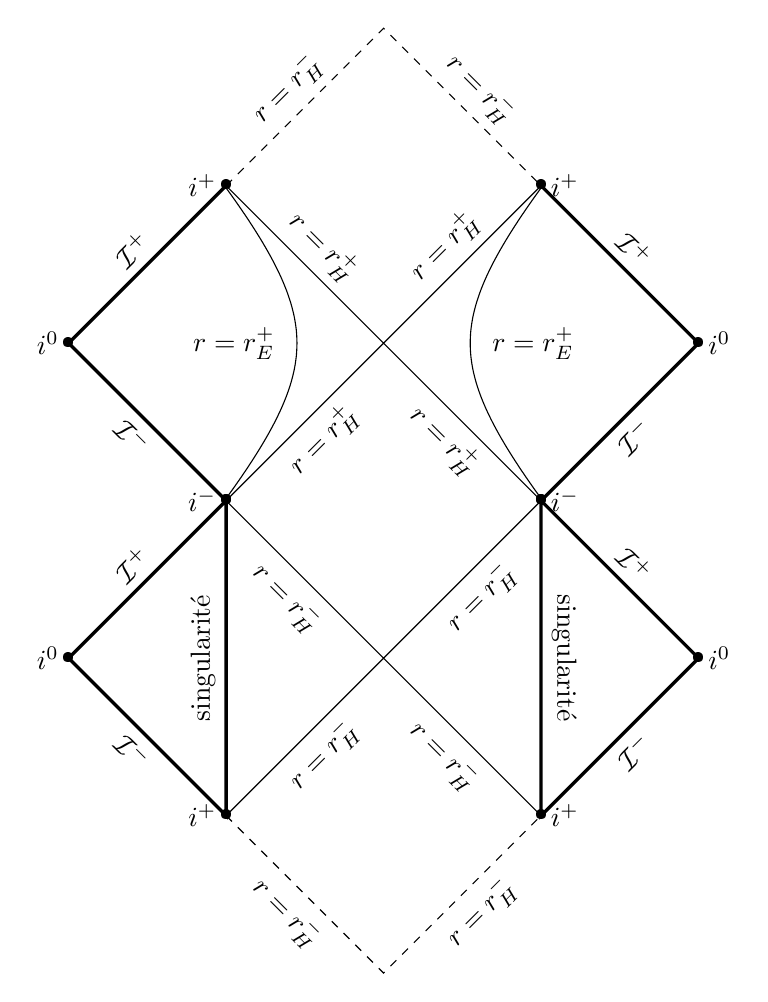
\begin{tikzpicture}
                \draw (-4,2) -- (-2,0) node[midway,below,rotate=-45]{$\mathcal{I^-}$} -- (0,2) node[midway,below,rotate=45]{$r=r^+_H$} -- (2,0) node[midway,below,rotate=-45]{$r=r^+_H$} -- (4,2) node[midway,below,rotate=45]{$\mathcal{I^-}$};
                \draw (-4,2) -- (-2,4) node[midway,above,rotate=45]{$\mathcal{I^+}$} -- (0,2) node[midway,above,rotate=-45]{$r=r^+_H$} -- (2,4) node[midway,above,rotate=45]{$r=r^+_H$} -- (4,2) node[midway,above,rotate=-45]{$\mathcal{I^+}$};
                \draw[dashed] (-2,4) -- (0,6) node[midway,above,rotate=45]{$r=r^-_H$} -- (2,4) node[midway,above,rotate=-45]{$r=r^-_H$};
                \draw[very thick] (-2,0) node{\textbullet} -- (-4,2) node{\textbullet} -- (-2,4) node{\textbullet};
                \draw[very thick] (2,0) node{\textbullet} -- (4,2) node{\textbullet} -- (2,4) node{\textbullet};
                
                \draw (-4,-2) -- (-2,0) node[midway,above,rotate=45]{$\mathcal{I^+}$} -- (0,-2) node[midway,below,rotate=-45]{$r=r^-_H$} -- (2,0) node[midway,below,rotate=45]{$r=r^-_H$} -- (4,-2) node[midway,above,rotate=-45]{$\mathcal{I^+}$};
                \draw (-4,-2) -- (-2,-4) node[midway,below,rotate=-45]{$\mathcal{I^-}$} -- (0,-2) node[midway,below,rotate=45]{$r=r^-_H$} -- (2,-4) node[midway,below,rotate=-45]{$r=r^-_H$} -- (4,-2) node[midway,below,rotate=45]{$\mathcal{I^-}$};
                \draw[dashed] (-2,-4) -- (0,-6) node[midway,below,rotate=-45]{$r=r^-_H$} -- (2,-4) node[midway,below,rotate=45]{$r=r^-_H$};
                \draw[very thick] (-2,0) node{\textbullet} -- (-4,-2) node{\textbullet} -- (-2,-4) node{\textbullet} -- (-2,0) node[midway,above,rotate=90]{singularité};
                \draw[very thick] (2,0) node{\textbullet} -- (4,-2) node{\textbullet} -- (2,-4) node{\textbullet} -- (2,0) node[midway,above,rotate=-90]{singularité};
                \draw (-2,0) node[left]{$i^-$};
                \draw (2,0) node[right]{$i^-$};
                \draw (-4,2) node[left]{$i^0$};
                \draw (4,2) node[right]{$i^0$};
                \draw (-2,4) node[left]{$i^+$};
                \draw (2,4) node[right]{$i^+$};
                \draw (-4,-2) node[left]{$i^0$};
                \draw (4,-2) node[right]{$i^0$};
                \draw (-2,-4) node[left]{$i^+$};
                \draw (2,-4) node[right]{$i^+$};
                \draw[domain=-2:2,smooth,variable=\x] plot({sqrt(1.3^2+0.9^2*\x*\x))-0.2},{\x+2});
                \draw[domain=-2:2,smooth,variable=\x] plot({-sqrt(1.3^2+0.9^2*\x*\x))+0.2},{\x+2});
                \draw (1.9,2) node{$r=r^+_E$};
                \draw (-1.9,2) node{$r=r^+_E$};
            \end{tikzpicture}
            \caption{Diagramme conforme de l'espace-temps de Kerr}
            \label{fig:my_label}
        \end{figure}